\ifgerman{\chapter{Evaluierung}}{\chapter{Evaluation}}
\label{ch:evaluation}

Evaluating a classification algorithm also known as classification model is necessary to find how competent the algorithm is on data it has never seen. The classification model generates probabilities when given the of predicting on unobserved data. 

\section{Experimental Setup}
Most of the experiments were carried out on \textit{Google Colab} is a free google service that provides Jupyter notebooks with Python environment that stores the notebooks on Google Drive. It provides a GPU (Graphics Processing Unit) or TPU (Tensor Processing Unit) and has pre-installed various popular machine learning and deep learning framework. The exact detail of the system is listed in the \ref{table:HWsetup}

\begin{table}[!ht]
\centering
\begin{tabular}{cc}
\hline
\textbf{Hardware} & \textbf{Specifications} \\ \hline
CPU & 2vCPU Intel(R) Xeon(R) Processors @2.20Ghz \\
GPU & 1xTesla K80 12GB(11.439GB Usable) GDDR5  VideoRAM \\
TPU & \multicolumn{1}{l}{Google's custom developed application-specific integrated circuits} \\
RAM & 12GB \\
DISK & 358.27 GB \\ \hline
\end{tabular}
\caption{Hardware specification for the experimental setup}
\label{table:HWsetup}
\end{table}

All the experiments were performed using \textit{Python 3} environment. \textit{scikit-learn}, an open source machine learning library in Python is used here for data processing and training the SVM. For Bidirectional LSTMs, \textit{Keras} an open source neural network library written in Python is used with \textit{Tensorflow} backend.  

The packages, their version numbers and the purpose are listed below in \ref{tabel:packageList}
\clearpage
\begin{table}[!ht]
\centering
\begin{tabular}{>{\centering\arraybackslash}m{3.4cm}>{\centering\arraybackslash}m{3.4cm}>{\centering\arraybackslash}m{6cm}}
\hline
\textbf{Package Name} & \textbf{Version Number} & \textbf{Description} \\ \hline
scikit-learn & 0.20.3 & An open source machine learning library for data mining and data analysis. \\[0.2cm]
keras & 2.2.4 & An open source neural network library for fast prototyping, uses likes of Tensorflow or Theano. \\[0.2cm]
tensorflow & 1.13.1 & An open source software library for numerical computation using data flow graphs. \\[0.2cm]
beautifulsoup4 & 4.6.3 & A python library for parsing HTML and XML documents. \\[0.2cm]
matplotlib & 3.0.3 & A python library for plotting and visualization. \\[0.2cm]
nltk & 3.2.5 & A python library for statistical Natural Language Processing. \\[0.2cm]
seaborn & 0.7.1 & A python library for statistical data visualization. \\[0.2cm]
spacy & 2.0.18 & An open-source software library for advanced Natural Language Processing. \\[0.2cm]
numpy & 1.14.6 & An python library for creating and manipulating, large and multiple dimensional arrays. \\[0.2cm]
scipy & 1.1.0 & An python library for scientific and technical computing \\ \hline
\caption{List of packages used}
\label{tabel:packageList}
\end{tabular}
\end{table}


\section{Evaluation Approach}
For evaluation, initially 70\% of data is used for training the classification models and then 30\% of the data is used for evaluation. The evaluation is done on sentence 

\begin{figure}[!ht]
    \centering
    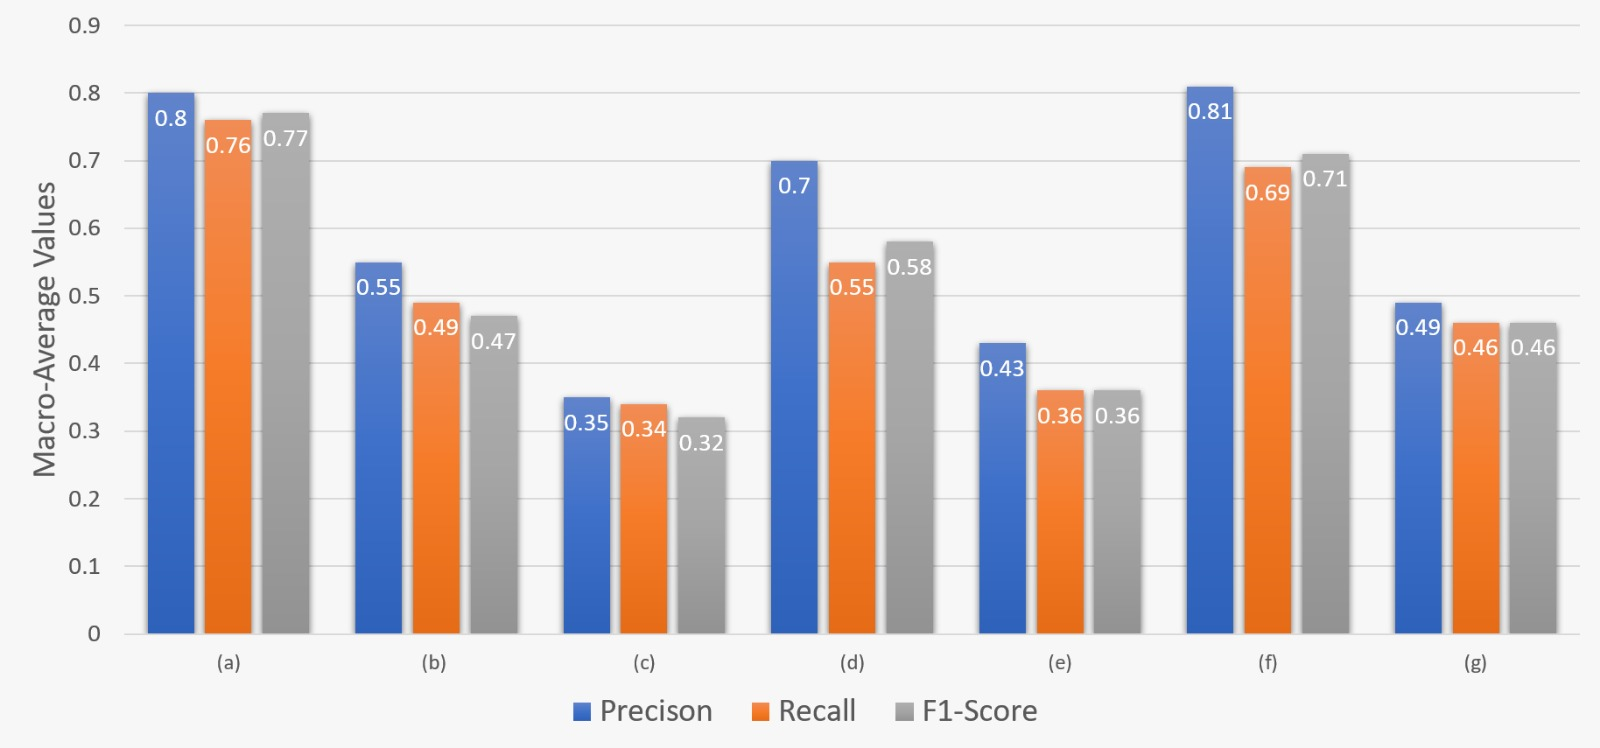
\includegraphics[width=16cm, keepaspectratio]{pics/EvaluationQ1.jpeg}
    \caption{Macro-averaged Precision, Recall and F1-Score of (a) Support Vector Machine on English data, (b) Bidirectional LSTM on English language without clustered data evaluated on document level, (c) Bidirectional LSTM on English language without clustered data, evaluated on sentence level, (d) Bidirectional LSTM on English and German language without clustered data, evaluated on document level, (e)
    Bidirectional LSTM on English and German language without clustered data, evaluated on sentence level, (f)
    Bidirectional LSTM on English and German language with clustered data, evaluated on document level, micro-average precision is the average of micro-average precision from cluster 1 and cluster 2  (g) Bidirectional LSTM on English and German language with clustered data, evaluated on sentence level, micro-average precision is the average of micro-average precision from cluster 1 and cluster 2}
    \label{fig:my_label}
\end{figure}